\documentclass[border=10pt]{standalone}
\usepackage[svgnames]{xcolor}
\usepackage{amsmath}
\usepackage{pgfplots}
\pgfplotsset{compat=newest}
\usepackage[sfdefault]{FiraSans}
\usepackage{FiraMono}
\renewcommand*\familydefault{\sfdefault}
\begin{document}
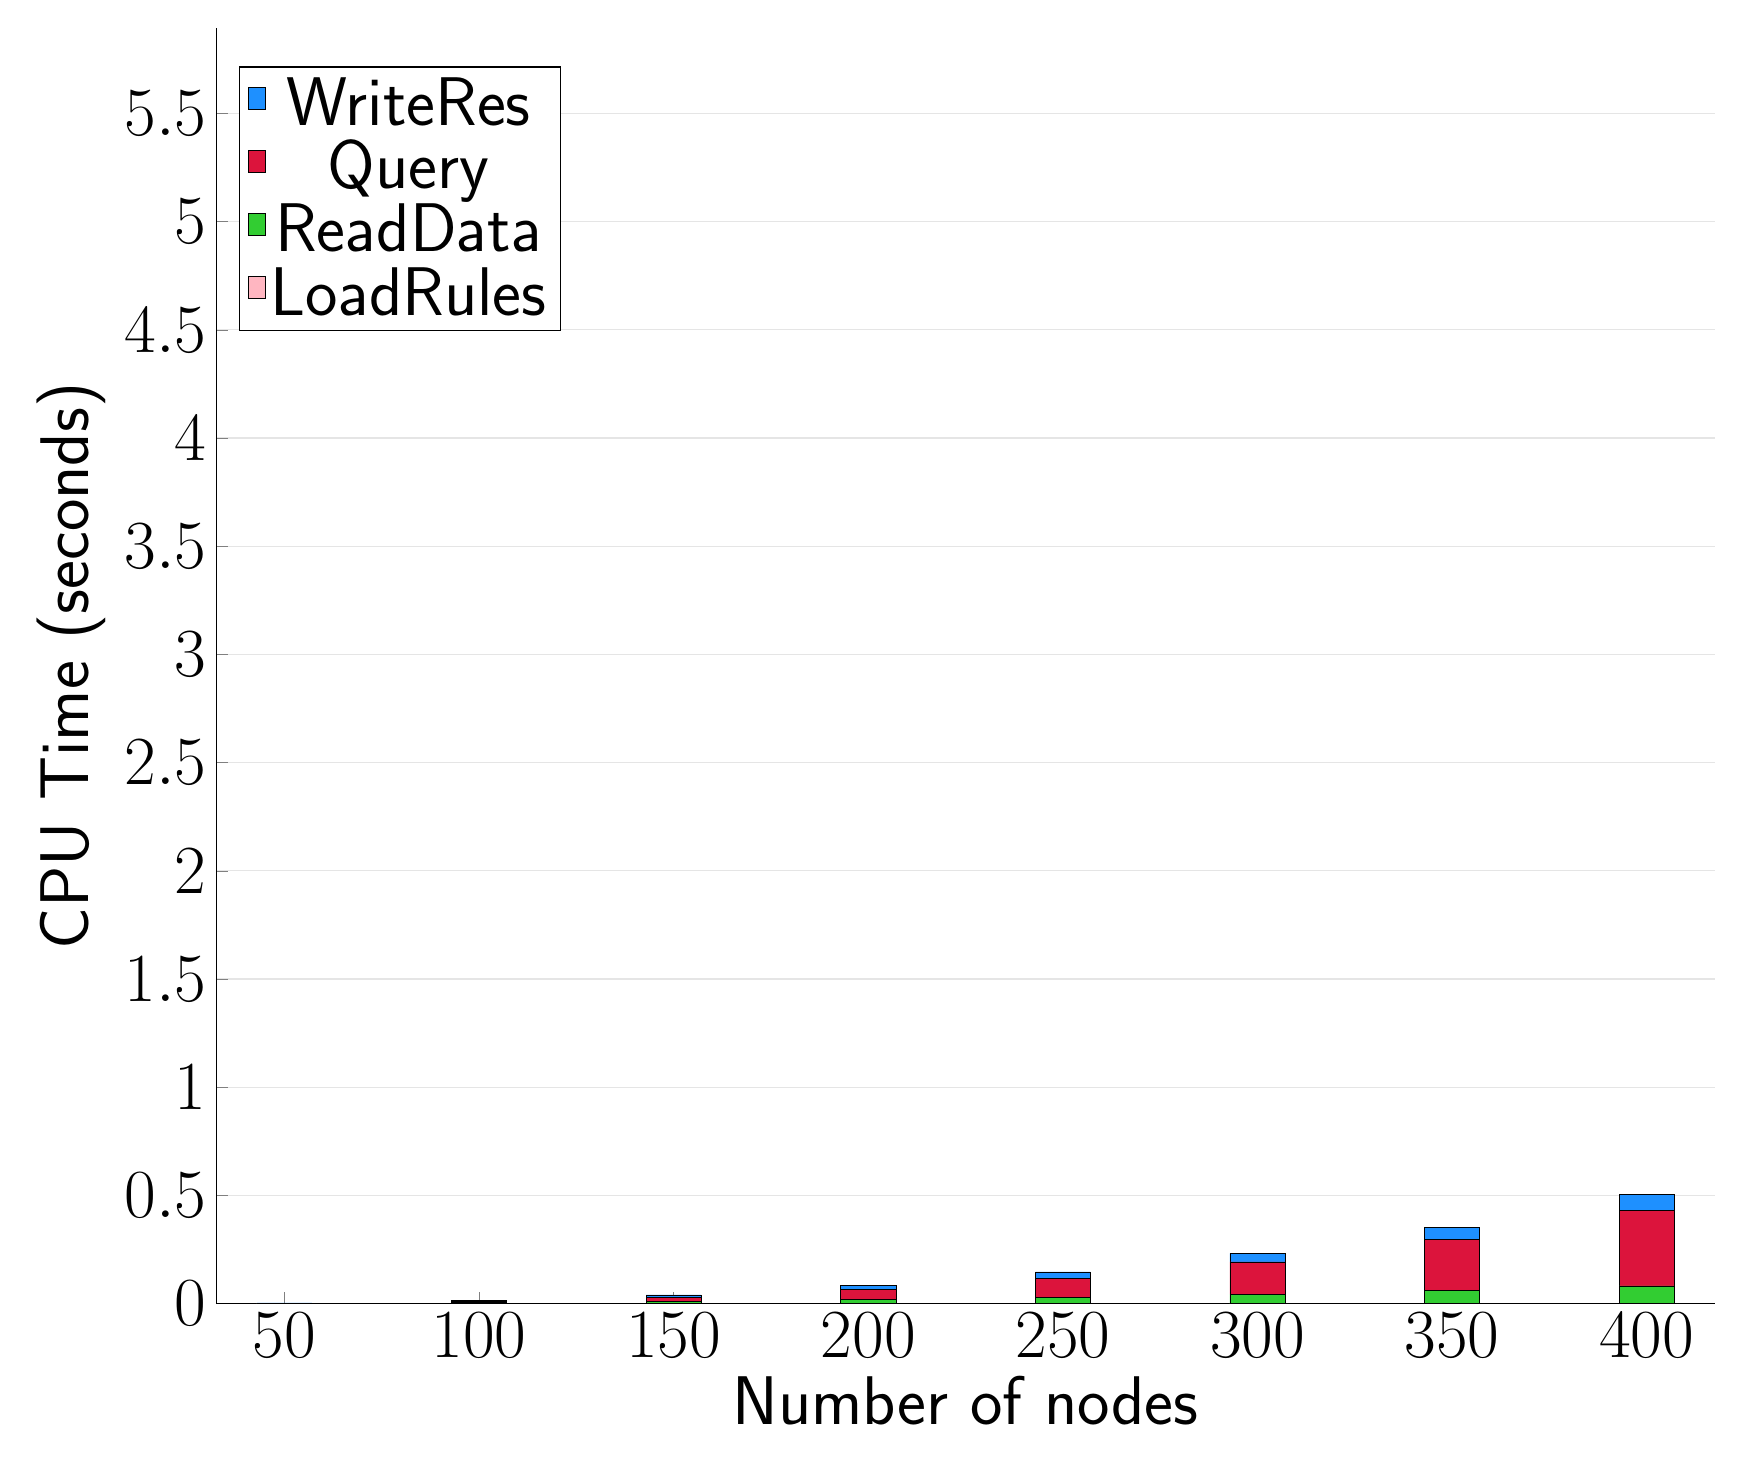
\begin{tikzpicture}
\begin{axis}[
   ybar stacked,
   width=1.7\textwidth,
   bar width=0.7cm,
   ymajorgrids, tick align=inside,
   major grid style={draw=gray!20},
   xtick=data,
   ymin=0, ymax=5.893940000000001,
   axis x line*=bottom,
   axis y line*=left,
   enlarge x limits=0.05,
   legend style={
       at={(0.23, 0.97)},
       anchor=north east,
       legend columns=1,
       font=\Huge,
   },
   ylabel={CPU Time (seconds)},
   xlabel={Number of nodes},
   label style={font=\Huge},
   tick label style={font=\Huge},
]
\addlegendimage{fill=DodgerBlue, draw=black, line width=0.2pt}
\addlegendentry{WriteRes}
\addlegendimage{fill=Crimson, draw=black, line width=0.2pt}
\addlegendentry{Query}
\addlegendimage{fill=LimeGreen, draw=black, line width=0.2pt}
\addlegendentry{ReadData}
\addlegendimage{fill=LightPink, draw=black, line width=0.2pt}
\addlegendentry{LoadRules}
\addplot +[fill=LightPink, draw=black, line width=0.2pt] coordinates {
(50, 0.0006081000000000005)
(100, 0.0006204000000000001)
(150, 0.0006104000000000002)
(200, 0.0006000000000000001)
(250, 0.0006129000000000004)
(300, 0.0006057999999999993)
(350, 0.0006081999999999999)
(400, 0.0006078000000000006)
};
\addplot +[fill=LimeGreen, draw=black, line width=0.2pt] coordinates {
(50, 0.0011595999999999998)
(100, 0.004443000000000001)
(150, 0.0102165)
(200, 0.0185578)
(250, 0.029586499999999995)
(300, 0.04339439999999999)
(350, 0.060472399999999996)
(400, 0.0808092)
};
\addplot +[fill=Crimson, draw=black, line width=0.2pt] coordinates {
(50, 0.0007838000000000001)
(100, 0.0057867)
(150, 0.019170200000000002)
(200, 0.04508739999999999)
(250, 0.0869516)
(300, 0.1490527)
(350, 0.2363366)
(400, 0.3505347)
};
\addplot +[fill=DodgerBlue, draw=black, line width=0.2pt] coordinates {
(50, 0.0011656)
(100, 0.004712200000000001)
(150, 0.0099514)
(200, 0.018474)
(250, 0.029002400000000005)
(300, 0.0389818)
(350, 0.05641630000000001)
(400, 0.0727807)
};
\end{axis}
\end{tikzpicture}

\end{document}
